\chapter{Algorytm DMC w wersji klasycznej}

\section{Pe�ny algorytm DMC}

Zaimplementowali�my r�wnie� algorytm DMC w wersji klasycznej (tj. wyznaczaj�cy trajektori� sterowania na ca�ym horyzoncie sterowania). Sprawdzili�my jego dzia�anie dla zestawu tych parametr�w, kt�re otrzymal�my w wyniku rozwi�zania zadania optymalizacji w poprzednim punkcie:

\begin{center}
\begin{tabular}{ | c | c | } \hline
$D$ & 150 \\ \hline 
$N$ & 25 \\ \hline 
$N_\mathrm{u}$ & 10 \\ \hline 
$\psi_\mathrm{1}$     &  \num{-85.49} \\ \hline    
$\psi_\mathrm{2}$     &  \num{8.47} \\ \hline  
$\psi_\mathrm{3}$     &  \num{8.72} \\ \hline  
$\lambda_\mathrm{1}$  &  \num{-3.21} \\ \hline  
$\lambda_\mathrm{2}$  &  \num{-9.05} \\ \hline  
$\lambda_\mathrm{3}$  &  \num{-0.26}\\ \hline  
$\lambda_\mathrm{4}$  &  \num{4.33} \\ \hline  
\end{tabular} 
\end{center}

Wyniki symulacji s� widoczne na rys.~\ref{DMCfull}. Warto�� wska�nika jako�ci $E=\num{510.1986}$.

\begin{figure}[tb]
	\centering
	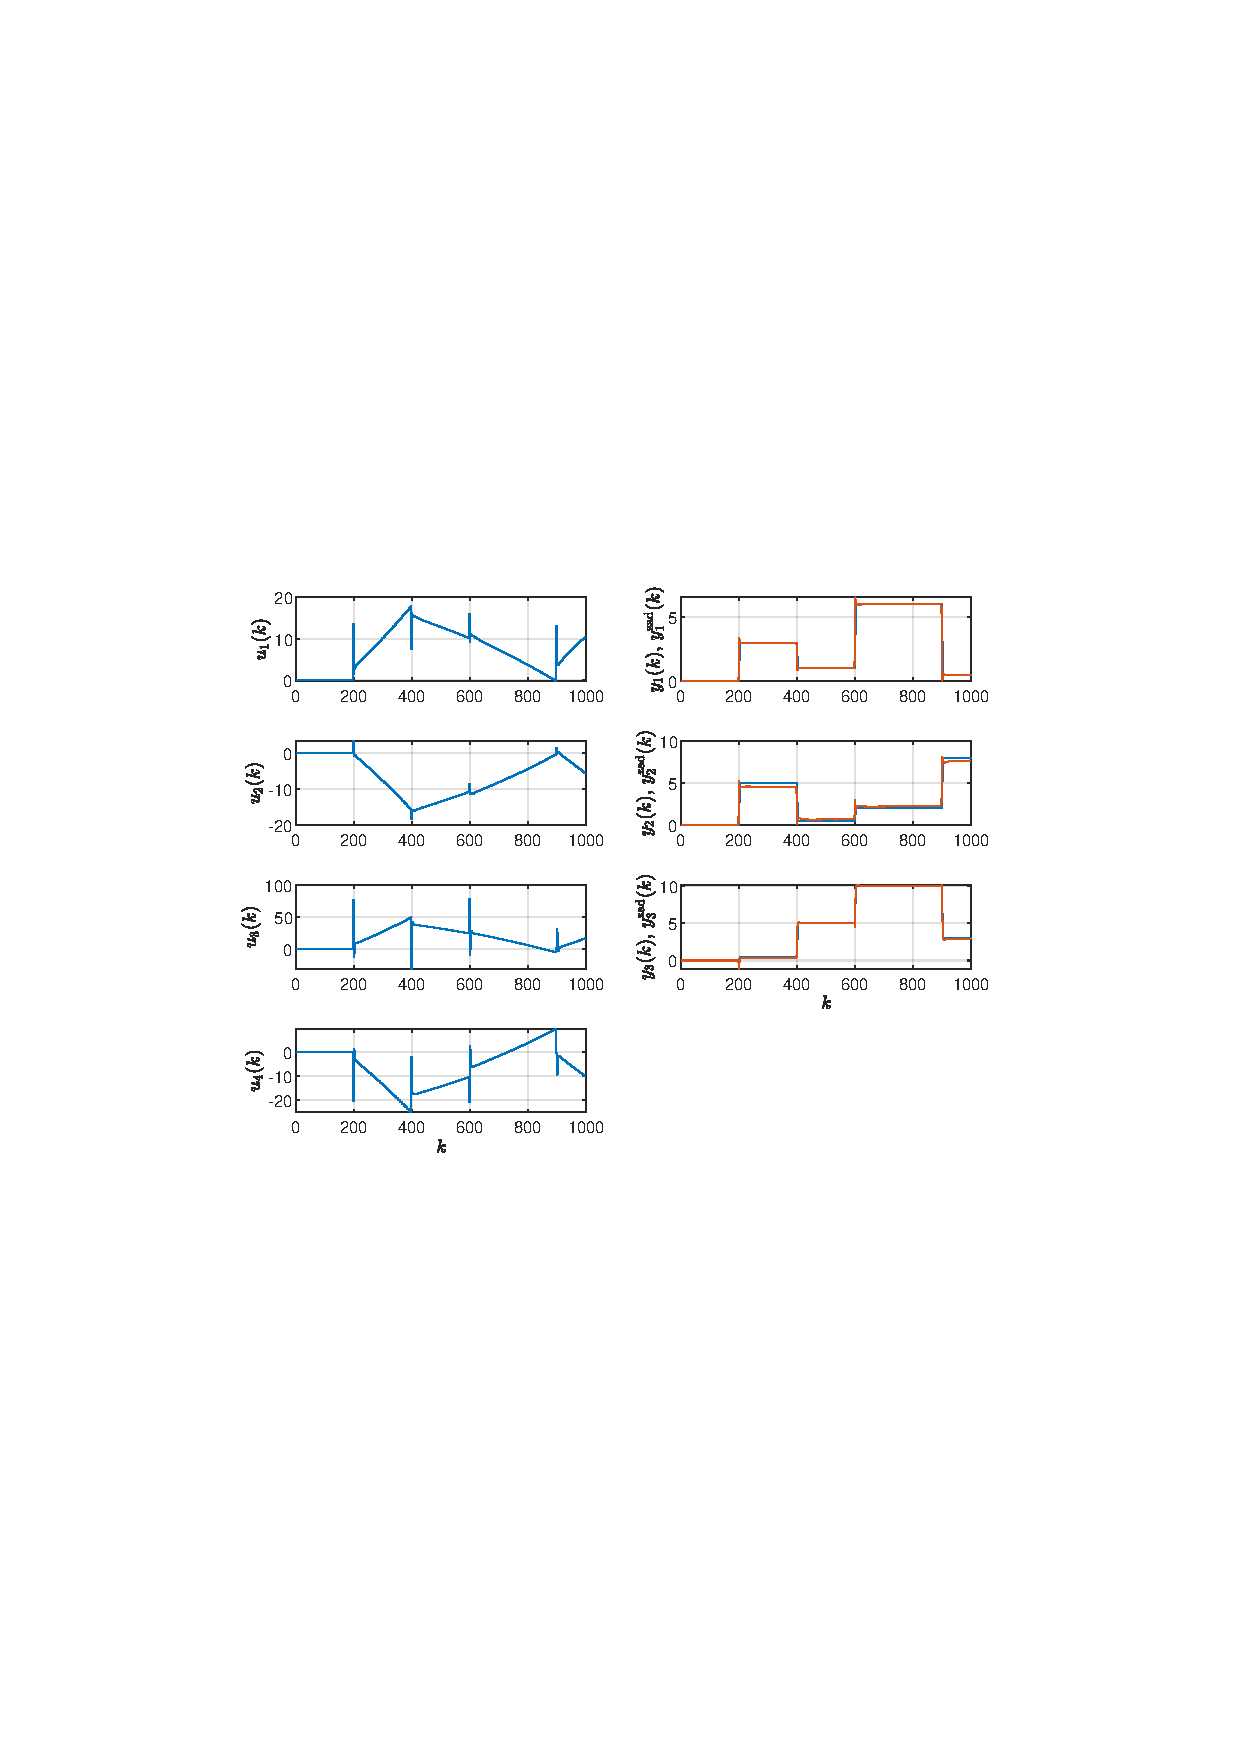
\includegraphics[scale=1, trim={2cm 8.5cm 2cm 8.5cm}]{rysunki/zad6_DMC_full}
	\caption{Regulacja DMC obiektu wielowymiarowego, $E=\num{510.1986}$ }
	\label{DMCfull}
\end{figure}

Otrzymane wyniki symulacji dla ustalonego zestawu parametr�w s� takie same zar�wno dla wersji pe�nej algorytmu DMC jak i dla wersji oszcz�dnej algorytmu DMC. Oznacza to, �e wypracowane przez nas rozwi�zanie jest poprawne.


\section{Implementacje}
Pe�ny algorytm DMC zaimplementowali�my w skrypcie \verb+DMC_full.m+.